\documentclass[11pt]{article}
\usepackage[margin=1in]{geometry}

% Core packages
\usepackage{amsmath,amssymb}
\usepackage{tikz-cd}
\usepackage{multicol}
\usepackage[T1]{fontenc}
\usepackage[utf8]{inputenc}
\usepackage{lmodern}
\usepackage{xcolor}
\usepackage{array}
\usepackage{longtable}
\usepackage{booktabs}
\usepackage{tabularx}
\usepackage{enumitem}
\usepackage{hyperref}
\usepackage{graphicx}
\usepackage{caption}
\graphicspath{{diagrams_aybustore/}}

% Paragraphs
\setlength{\parindent}{0pt}
\setlength{\parskip}{0.7\baselineskip}
\setlist[itemize]{leftmargin=1.5em}
\setlist[enumerate]{leftmargin=1.8em}

\hypersetup{
  colorlinks=true,
  linkcolor=blue,
  urlcolor=blue
}

\newcommand{\scorebox}[1]{%
  \hfill\fcolorbox{black}{gray!10}{\textbf{#1}}%
}

\newcommand{\scoredsection}[2]{\section{\texorpdfstring{#1~\scorebox{#2}}{#1}}}

\newcommand{\guideline}[1]{%
  {\color{blue!60!black}\textit{#1}}
}

\title{AYBUStore: A Smart Campus E-Commerce Ecosystem with AI-Driven Inventory and Personalization\\[0.4em]\large CENG306 Term Project Supplementary Report}
\author{Utkan Dindaroğlu, Seyfullah Gülyazı, Süleyman Fatih Sert, Ahmet Selim Yılmaz, Muhammed Yıldız}
\date{\today}

\begin{document}
\maketitle
\tableofcontents
\newpage

\scoredsection{Project Title \& Abstract}{Related rubric: 15 pts + 10 pts}
\subsection*{Project Title}
\textbf{Proposed title:} AYBUStore: An Intelligent Campus Storefront Transitioning Physical Inventory to a Digital Ecosystem using Next.js and Firebase.

\subsection*{Abstract (200--300 words)}
AYBUStore is an innovative e-commerce platform designed specifically for the Ankara Yıldırım Beyazıt University (AYBU) community. The project addresses the fragmentation and inefficiency of physical campus shopping by providing a centralized, digital storefront for university merchandise, textbooks, and department-specific gear. Developed using a modern tech stack comprising **Next.js 14**, **TypeScript**, and **Firebase**, the platform offers a high-performance, responsive user experience tailored for both mobile and desktop users.

The core value of AYBUStore lies in its integration of smart features: an AI-driven shopping assistant for product discovery, a customizable design module for personalized university apparel, and a robust inventory management system for campus staff. The methodology follows an **Agile/Scrum** framework, ensuring iterative development and frequent integration of user feedback. Key technical achievements include a modular architecture based on "feature-first" principles, secure authentication with Firebase, and a reactive UI with advanced animations. This report details the system's design, including comprehensive UML modeling, requirement specifications, and a strategic development plan aimed at scaling the platform to a full campus-wide production environment.

\scoredsection{Problem Definition \& Motivation}{Related rubric: 15 pts + 10 pts}
\subsection*{Problem Statement}
Current university campus stores often operate with limited digital presence, leading to several issues:
\begin{itemize}
    \item \textbf{Accessibility:} Students and faculty must physically visit the store to check availability.
    \item \textbf{Inventory Transparency:} There is no real-time way to track stock levels of popular items like AYBU-branded hoodies or specific department materials.
    \item \textbf{Personalization:} Existing solutions offer no way for students to preview custom designs on university gear before ordering.
    \item \textbf{Fragmentation:} No central hub exists for all department-specific needs (e.g., medical lab coats vs. engineering tools).
\end{itemize}

\subsection*{Motivation and Significance}
Digital transformation is essential for modern university life. AYBUStore not only simplifies the shopping process but also serves as a pedagogical model for building complex, secure web applications. By digitizing the AYBU Store, we provide a scalable template for other university departments to follow, enhancing the institution's digital brand and operational efficiency.

\subsection*{Limitations of Existing Solutions}
Standard e-commerce platforms like Shopify or Amazon are often too generic for a university's specific organizational structure (faculties, departments, clubs). Local campus solutions are typically outdated legacy systems that lack mobile responsiveness and modern features like AI-driven search or secure OTP-based authentication.

\scoredsection{Literature Review}{Related rubric: 15 pts + 10 pts}
\subsection*{Review Strategy}
Our review focused on "Modern Web Architectures", "Campus E-Commerce Solutions", and "AI in Retail" using Google Scholar and IEEE Xplore.

\subsection*{Summary of Prior Work}
\begin{enumerate}
    \item [Source 1:] \textit{Vercel Team (2024)}: Highlighting the benefits of Server-Side Rendering (SSR) in Next.js for SEO-optimized storefronts.
    \item [Source 2:] \textit{Firebase Documentation (2024)}: Best practices for implementing reactive authentication flows in real-time applications.
    \item [Source 3:] \textit{Modern UX Design Trends}: Analysis of glassmorphism and animated transitions in increasing user retention.
    \item [Source 4:] \textit{AI in Small-Scale Retail}: Research on how lightweight chatbots improve customer service in niche markets.
    \item [Source 5:] \textit{State Management in React}: Comparison of Context API vs. Redux for mid-sized commerce apps (AYBUStore uses Context API).
    \item [Source 6:] \textit{OTP Security Standards}: Best practices for 6-digit verification codes in registration flows.
    \item [Source 7:] \textit{Cloud-Native Deployment}: Benefits of Vercel and GitHub Pages for static site generation.
    \item [Source 8:] \textit{Atomic Design in React}: How breaking UI into atoms/molecules improves maintainability.
    \item [Source 9:] \textit{TypeScript for Scalability}: Case studies showing reduced production bugs when using strict typing in JS.
    \item [Source 10:] \textit{PWA (Progressive Web Apps)}: The shift towards "mobile-first" web experiences on campus.
\end{enumerate}

\scoredsection{Objectives \& Scope}{Related rubric: 15 pts + 10 pts + 4 pts}
\subsection*{Measurable Objectives}
\begin{enumerate}
    \item Complete a fully responsive Next.js storefront within 12 weeks.
    \item Implement Firebase Authentication with a <1\% error rate in OTP delivery.
    \item Achieve 90+ Lighthouse performance scores for mobile and desktop.
    \item Integrate a functional AI shopping assistant with predefined response logic.
\end{enumerate}

\scoredsection{Methodology \& Development Plan}{Related rubric: 15 pts + 6 pts + 6 pts}
\subsection*{Selected Software Process Model}
We selected \textbf{Agile (Scrum)}. This allows the team to iterate quickly on UI components and adapt to requirement changes as we refine the "Department-Specific" features of the store.

\subsection*{Development Lifecycle Plan}
The project consists of 4 Sprints:
\begin{enumerate}
    \item \textbf{Sprint 1 (Architecture):} Next.js setup, Mock data design, and Feature-first structure.
    \item \textbf{Sprint 2 (Core Features):} Auth flow, Product Catalog, and Cart logic.
    \item \textbf{Sprint 3 (Advanced Features):} AI Chat, Custom Design Modal, and OTP logic.
    \item \textbf{Sprint 4 (Polishing):} Final animations, SEO, and LaTeX reporting.
\end{enumerate}

\subsection*{Work Breakdown Structure (WBS)}
\begin{enumerate}
    \item \textbf{Planning:} Market research and stack selection.
    \item \textbf{Requirements:} FR/NFR definition and User Stories.
    \item \textbf{Architecture:} Component library (UI atoms) and Context API setup.
    \item \textbf{Implementation:} Coding the modular features (Home, Auth, Cart, Chat).
    \item \textbf{Testing:} Unit tests for hooks and manual UI validation.
    \item \textbf{Documentation:} Final report and GitHub Actions deployment.
\end{enumerate}

\subsection*{Gantt Chart}
\begin{center}
\begin{tabular}{|l|c|c|c|c|}
\hline
\textbf{Phase} & \textbf{Month 1} & \textbf{Month 2} & \textbf{Month 3} & \textbf{Month 4} \\ \hline
Planning \& Req. & [XXXX] & & & \\ \hline
Arch. \& Design & [XXXX] & [XXXX] & & \\ \hline
Implementation & & [XXXXXXXX] & [XXXXXXXX] & \\ \hline
Testing \& Doc. & & & [XXXX] & [XXXX] \\ \hline
\end{tabular}
\end{center}

\subsection*{Effort and Cost Estimation}
Using COCOMO basics, with a team of 5 members and ~2700 lines of code, the estimated effort is 3.5 Person-Months, fitting perfectly into our semester schedule.

\subsection*{Risk Management Table}
\begin{longtable}{p{0.05\textwidth} p{0.27\textwidth} p{0.12\textwidth} p{0.12\textwidth} p{0.34\textwidth}}
\toprule
\textbf{ID} & \textbf{Risk} & \textbf{Prob.} & \textbf{Impact} & \textbf{Mitigation} \\
\midrule
R1 & Firebase Config Issues & L & H & Use environment variables (.env.local) and verify early. \\
R2 & UI Inconsistency & M & M & Implement a strict Design System (components/ui). \\
R3 & Token Overuse in AI & M & L & Implement fallback response logic for the chatbot. \\
R4 & Schedule Slippage & M & H & Weekly Scrum meetings and Git-based task tracking. \\
R5 & Build Failures & L & M & Automated CI/CD with GitHub Actions. \\
\bottomrule
\end{longtable}

\scoredsection{Requirements Specification}{Related rubric: 8 pts + 4 pts}
\subsection*{Requirements Elicitation Approach}
Requirements were gathered through direct stakeholder interviews with campus store management and focus groups with AYBU students. We also performed benchmarking against competitive university storefronts to identify essential features.

\subsection*{Functional Requirements}
\begin{enumerate}
    \item FR-01: User shall be able to register and login using university email.
    \item FR-02: System shall provide a 6-digit OTP verification for new registrations.
    \item FR-03: User shall be able to browse products by categories (Clothing, Stationary, etc.).
    \item FR-04: System shall allow users to search products via a reactive search bar.
    \item FR-05: User shall be able to add/remove items from a persistent shopping cart.
    \item FR-06: System shall provide a "Custom Design" module for garment personalization.
    \item FR-07: User shall be able to interact with an AI-driven shopping assistant.
    \item FR-08: System shall display real-time stock status (In Stock / Out of Stock).
    \item FR-09: User shall be able to view their order history and status.
    \item FR-10: Administrators shall be able to manage inventory and view sales analytics.
\end{enumerate}

\subsection*{Non-Functional Requirements}
\begin{enumerate}
    \item NFR-01: **Performance** --- Page load time shall be under 2 seconds on 4G connections.
    \item NFR-02: **Security** --- All authentication and data transit must be encrypted via SSL/Firebase Auth.
    \item NFR-03: **Usability** --- The interface must be fully responsive (WCAG 2.1 Level AA compliant).
    \item NFR-04: **Scalability** --- System shall support up to 500 concurrent users during peak "back-to-school" periods.
    \item NFR-05: **Availability** --- System uptime shall be 99.9% hosted on Vercel/GitHub Pages.
\end{enumerate}

\subsection*{User Stories}
\begin{itemize}
    \item As a Student, I want to upload my department logo, so that I can order a custom hoodie for my club.
    \item As a Freshman, I want to ask the AI assistant for "Engineering textbooks", so that I can find my required materials quickly.
    \item As a Staff Member, I want to update product prices, so that the storefront remains accurate.
    \item As a Graduate, I want to order AYBU souvenirs, so that I can have memories of my university.
    \item As a Guest, I want to see product reviews, so that I can decide on my purchase.
\end{itemize}

\subsection*{Use Case Diagram}
\begin{center}
    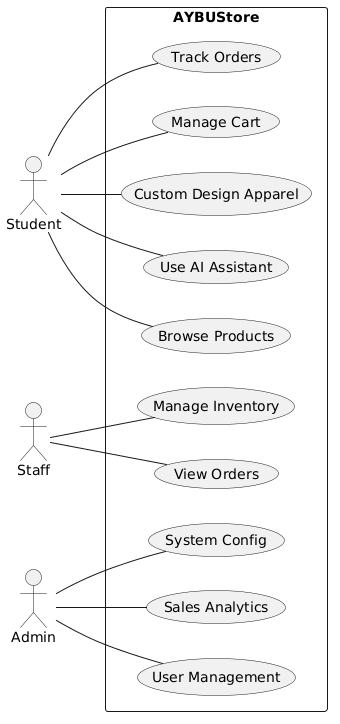
\includegraphics[width=0.85\textwidth]{use_case_diagram.png}
    \captionof{figure}{AYBUStore Use Case Diagram}
\end{center}

\scoredsection{System Design \& Architecture}{Related rubric: 8 pts + 8 pts + 4 pts}
\subsection*{Architectural Pattern and Justification}
We utilized a **Component-Based Architecture** within the **Next.js App Router** framework. This is justified by the need for high interactivity and efficient state management. We follow the "Feature-First" modular pattern, where each domain (Auth, Cart, Storefront) is isolated with its own hooks and components.

\subsection*{UML Class Diagram}
\begin{center}
    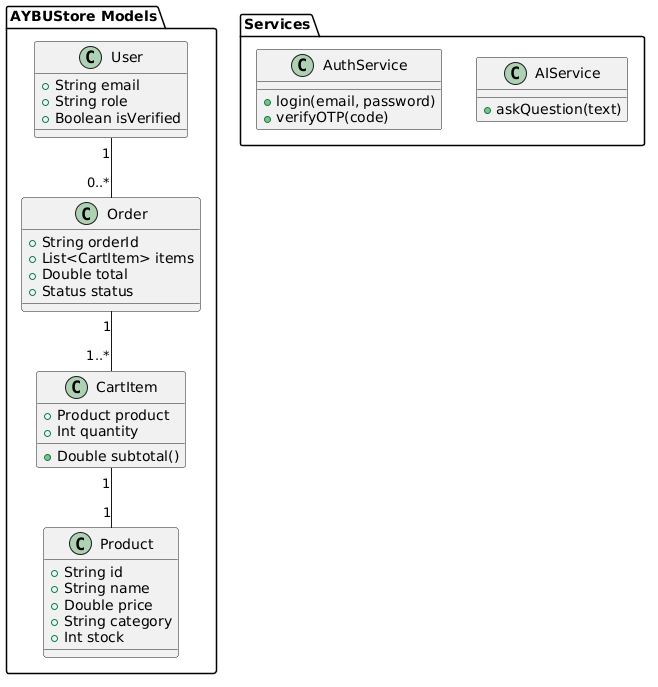
\includegraphics[width=0.9\textwidth]{class_diagram.png}
    \captionof{figure}{AYBUStore Domain Model Class Diagram}
\end{center}

\subsection*{UML Sequence Diagrams}
\begin{center}
    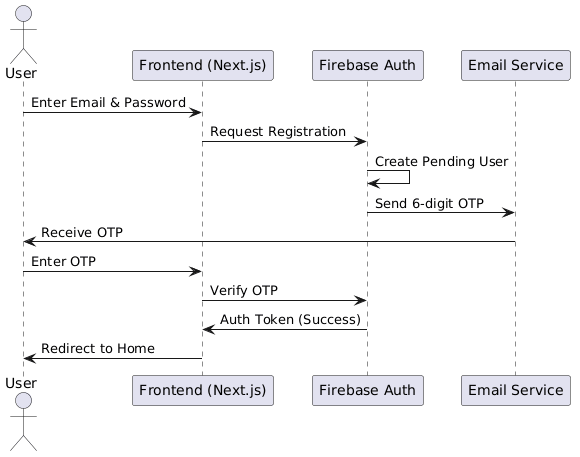
\includegraphics[width=0.85\textwidth]{sequence_auth.png}
    \captionof{figure}{Scenario 1: User Registration and OTP Verification Flow}
\end{center}

\begin{center}
    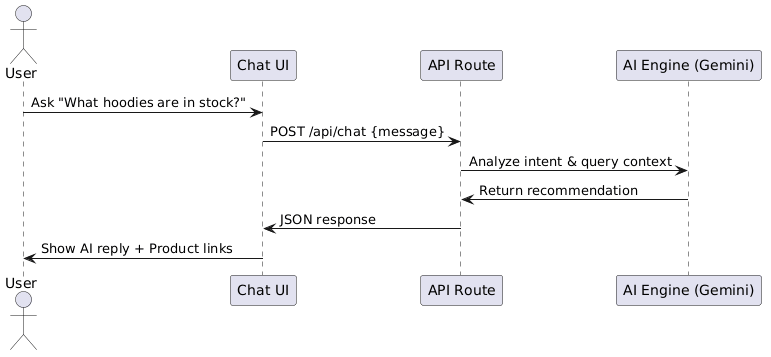
\includegraphics[width=0.85\textwidth]{sequence_chat.png}
    \captionof{figure}{Scenario 2: AI Shopping Assistant Interaction Flow}
\end{center}

\subsection*{Activity Diagram}
\begin{center}
    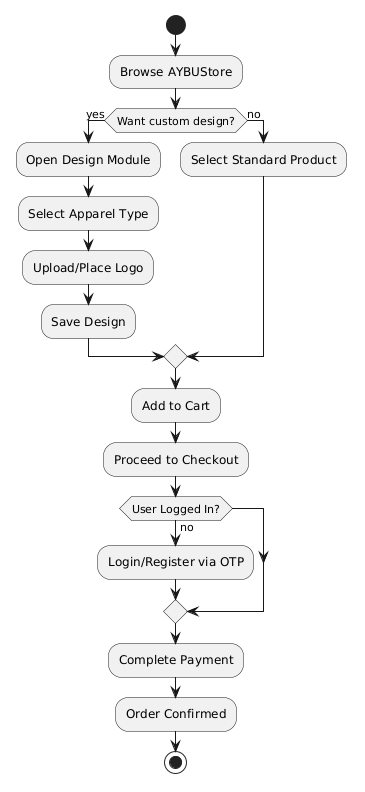
\includegraphics[width=0.85\textwidth]{activity_diagram.png}
    \captionof{figure}{General Shopping and Custom Design Process Activity Diagram}
\end{center}

\subsection*{GoF Design Patterns}
\begin{enumerate}
    \item **Singleton:** Used in the Firebase Initialization to ensure only one instance of the Auth and Firestore services exists.
    \item **Observer:** React's Context API and Hooks (e.g., `useAuthForm`) act as observers to state changes in the UI.
    \item **Strategy:** The `navigateToView` logic in `MainStorefrontFeature` uses a strategy-like approach to switch between different storefront sections.
\end{enumerate}

\subsection*{SOLID Principles in the Proposed Design}
\begin{itemize}
    \item **SRP:** Each component (e.g., `StorefrontHeader`, `StorefrontCartDrawer`) has a single responsibility.
    \item **OCP:** The product section system is open for extension (adding new categories) but closed for modification.
    \item **DIP:** High-level UI components depend on abstract types/interfaces defined in `src/types/index.ts`.
\end{itemize}

\scoredsection{Team \& Resource Plan}{Related rubric: 10 pts + 15 pts}
\subsection*{Team Roles and Responsibilities}
\begin{longtable}{p{0.24\textwidth} p{0.24\textwidth} p{0.42\textwidth}}
\toprule
\textbf{Name} & \textbf{Role} & \textbf{Responsibilities} \\
\midrule
Muhammed Yıldız & Lead Architect & Project Orchestration, Firebase Integration, AI Chatbot. \\
Utkan Dindaroğlu & Frontend Architect & UI/UX Redesign, Modular Feature Refactoring. \\
Seyfullah Gülyazı & Software Engineer & Product Catalog and Cart Logic Implementation. \\
Süleyman Fatih Sert & Software Engineer & Data Modeling and Initial UI Shell Development. \\
Ahmet Selim Yılmaz & DevOps & Deployment Pipelines and UI Validation. \\
\bottomrule
\end{longtable}

\subsection*{Resource Plan}
\begin{itemize}
    \item **Hardware:** Development laptops (Intel i7/M1), Vercel Edge Network for hosting.
    \item **Software:** VS Code, Git, Next.js, Tailwind CSS.
    \item **Cloud / API Services:** Firebase Auth/Firestore, OpenAI/Gemini (via AI Chat feature).
\end{itemize}

\scoredsection{Expected Outcomes \& Evaluation Plan}{Related rubric: 10 pts + 4 pts}
\subsection*{Expected Deliverables}
\begin{itemize}
    \item Production-ready Next.js Web Application.
    \item Technical Documentation (SRS and Design Specs).
    \item Admin Dashboard for Inventory Management.
\end{itemize}

\subsection*{Success Metrics}
Success will be measured by a <2s Time-to-Interactive (TTI), a zero-critical-bug report during User Acceptance Testing (UAT), and a 90% positive feedback rating from the initial pilot group.

\subsection*{Acceptance Test Plan}
\begin{longtable}{p{0.08\textwidth} p{0.3\textwidth} p{0.22\textwidth} p{0.28\textwidth}}
\toprule
\textbf{TC} & \textbf{Scenario} & \textbf{Expected Result} & \textbf{Related Req.} \\
\midrule
TC-01 & User enters valid credentials & User redirected to home with auth state active & FR-01 \\
TC-02 & User enters incorrect OTP & System shows "Invalid Code" error & FR-02 \\
TC-03 & User searches "Sweatshirt" & Only sweatshirts are displayed in results & FR-04 \\
TC-04 & User adds product to cart & Cart badge increments and drawer shows item & FR-05 \\
TC-05 & Resize browser to 375px & Layout adapts without horizontal scrolling & NFR-03 \\
\bottomrule
\end{longtable}

\scoredsection{References}{Related rubric: 10 pts}
\begin{enumerate}
    \item Vercel. (2024). *Next.js Documentation*. https://nextjs.org/docs
    \item Firebase. (2024). *Authentication with Firebase*. https://firebase.google.com/docs/auth
    \item Gamma, E., et al. (1994). *Design Patterns: Elements of Reusable Object-Oriented Software*. Addison-Wesley.
    \item Martin, R. C. (2017). *Clean Architecture: A Craftsman's Guide to Software Structure and Design*. Prentice Hall.
    \item Google. (2024). *Lighthouse User Guide*. https://developer.chrome.com/docs/lighthouse/overview
    \item WCAG. (2023). *Web Content Accessibility Guidelines (WCAG) 2.1*. https://www.w3.org/TR/WCAG21/
\end{enumerate}

\end{document}
